\documentclass{beamer}

\usetheme{metropolis}

\usepackage{xparse}
\usepackage{xfrac}
\usepackage{xcolor}
\usepackage{cancel}
\usepackage{amssymb}
\usepackage{amsmath}
\usepackage{graphicx}
\usepackage{spalign}
\usepackage{multirow}
\usetikzlibrary{automata, arrows, positioning}

\definecolor{links}{HTML}{2A1B81}
\hypersetup{colorlinks,linkcolor=,urlcolor=links}

% https://tex.stackexchange.com/questions/2233/whats-the-best-way-make-an-augmented-coefficient-matrix
\makeatletter
\renewcommand*\env@matrix[1][*\c@MaxMatrixCols c]{%
  \hskip -\arraycolsep
  \let\@ifnextchar\new@ifnextchar
  \array{#1}}
\makeatother


% https://tex.stackexchange.com/questions/102069/make-a-heading-in-beamer
\newcommand\makeheader[1]{%
  \par\bigskip
  {\large\bfseries#1}\par\smallskip}


\ExplSyntaxOn
\NewDocumentCommand{\mat}{ O{b} m }
 {
  \strategy_matlabmatrix:nn { #1 } { #2 }
 }

\seq_new:N \l_strategy_rows_seq
\seq_new:N \l_strategy_a_row_seq
\tl_new:N \l_strategy_matrix_tl

\cs_new_protected:Npn \strategy_matlabmatrix:nn #1 #2
 {
  \tl_clear:N \l_strategy_matrix_tl
  \seq_set_split:Nnn \l_strategy_rows_seq { ; } { #2 }
  \seq_map_inline:Nn \l_strategy_rows_seq
   {
    \seq_set_split:Nnn \l_strategy_a_row_seq { ~ } { ##1 }
    \tl_put_right:Nx \l_strategy_matrix_tl { \seq_use:Nn \l_strategy_a_row_seq { & } }
    \tl_put_right:Nn \l_strategy_matrix_tl { \\ }
   }
  \begin{#1matrix}
  \tl_use:N \l_strategy_matrix_tl
  \end{#1matrix}
 }
\ExplSyntaxOff

\newenvironment{blueenv}{\only{\setbeamercolor{local structure}{fg=blue}}}{}


\usepackage[siunitx, american]{circuitikz}

%necessary to use pandoc's outputted latex itemize sections
\providecommand{\tightlist}{%
  \setlength{\itemsep}{0pt}\setlength{\parskip}{0pt}}



\title{EECS 16A Midterm 1 Review Session}
\author{Presented by \textless NAMES \textgreater (HKN)}
\date{}

\newcommand{\SlideAccessingLogistics}{@\#}
\newcommand{\SlidesLocation}{\href{https://hkn.mu/16Aslides}{hkn.mu/16Aslides}}
\newcommand{\PresenterHours}{\item Name 1: \begin{flushright} Time 1: \end{flushright}}


\begin{document}
\righthyphenmin=62
\providecommand{\SlideAccessingLogistics}{\textless Insert piazza post number here \textgreater}
\providecommand{\SlidesLocation}{\textless Slides location and/or link \textgreater}
\providecommand{\PresenterHours}{\textless Itemize the presenter hours here \textgreater}

\begin{frame}

\titlepage

\end{frame}

\begin{frame}[t]\vspace{20pt}
\frametitle{Disclaimer}
This is an unofficial review session and HKN is not affiliated with this course. Although some of the presenters may be course staff, the material covered in the review session may not be an accurate representation of the topics covered in and difficulty of the exam.

% If you want to follow along: head to \SlidesLocation

Slides are also posted at \SlideAccessingLogistics\ on Piazza.

\begin{footnotesize}
  This is licensed under the Creative Commons CC BY-SA: feel free to share and edit, as long as you credit us and keep the license. For more information, visit
  \href{https://creativecommons.org/licenses/by-sa/4.0/}{https://creativecommons.org/licenses/by-sa/4.0/}
\end{footnotesize}

\vspace{20pt}

\end{frame}


\begin{frame}[t]\vspace{20pt}
\frametitle{HKN Drop-In Tutoring}

\begin{itemize}
  \item HKN has office hours Monday through Friday from \textbf{1 PM - 5 PM} and \textbf{9 PM - 10 PM} on \href{https://hkn.mu/ohqueue}{hkn.mu/ohqueue} and in our Soda 345 and Cory 290 offices.
  \item The schedule of tutors can be found at \href{https://hkn.mu/tutor}{hkn.mu/tutor}
  % \PresenterHours
\end{itemize}

\end{frame}


\section{Matrices and Linear Transformations}

\begin{frame}{Matrices}
    \begin{itemize}
        \item Matrices are \textbf{collections of vectors}.
        \item Typically represent \textbf{systems of equations}, where each row is an equation and each column is a variable.
        \item Notable matrices:
        \begin{itemize}
            \item Identity matrix
            \begin{align*}
                \begin{bmatrix}
                    1 & 0 \\
                    0 & 1
                \end{bmatrix}
                \begin{bmatrix}
                    a & b \\
                    c & d
                \end{bmatrix} =
                \begin{bmatrix}
                    a & b \\
                    c & d
                \end{bmatrix} 
            \end{align*}
            \item Rotation matrix
            \begin{align*}
                \begin{bmatrix}
                    \cos(\theta) & -\sin(theta) \\
                    \sin(\theta) & \cos(\theta)
                \end{bmatrix}
            \end{align*}
        \end{itemize}
    \end{itemize}
\end{frame}

\begin{frame}{Augmented Matrices}
    \textbf{Augmented matrices} are a way of represening both sides of a system of equations using one matrix:
    \begin{align*}
        x - 2y + 3z = 7 \\
        2x + y + z = 4 \\
        -2x + 2y -2z = -10 \\
        \begin{bmatrix}[c c c | c]
            1 & -2 & 3 & 7 \\
            2 & 1 & 1 & 4 \\
            -2 & 2 & -2 & -10
        \end{bmatrix}
    \end{align*}
\end{frame}
\section{Gaussian Elimination}

\begin{frame}{Gaussian Elimination}

\end{frame}


\begin{frame}{Practice: Gaussian Elimination}

\end{frame}

\begin{frame}{Possible results of Gaussian Elimination on $A\vec{x} = \vec{b}$}

\end{frame}
\section{Linear Transformations}

\begin{frame}{Linear Transformations}
    \begin{itemize}
        \item \textbf{Linear transformations} are operations that can be performed by applying a matrix to a vector. 
        \item Some common transformations include \textbf{rotation} and \textbf{reflection}.
    \end{itemize}
    \begin{center}
        \includegraphics[width = 0.45\textwidth]{images/vector-rotation.png} 
        \includegraphics[width = 0.45\textwidth]{images/vector-reflection.png}
    \end{center}
\end{frame}

\begin{frame}{Common Linear Transformations: Rotation}
    The \textbf{rotation matrix} rotates points by a specific angle, $\theta$:
    \begin{align*}
        R(\theta) = \begin{bmatrix} 
                \cos(\theta) & -\sin(\theta) \\
                \sin(\theta) & \cos(\theta)
            \end{bmatrix}
    \end{align*}
    Use this matrix by \textbf{plugging in the desired rotation angle}, then multiply it to a vector.
    \begin{align*}
        R(\theta) = \begin{bmatrix} 
            0 & -1 \\
            1 & 0
        \end{bmatrix}
    \end{align*}
    Rotation matrices also \textbf{preserve the length} of a vector. Check it! (\textit{Think about the eigenvalues! Real? Complex? How about the magnitude of these eigenvalues?})
\end{frame}

\begin{frame}{Common Linear Transformations: Reflection}
    \begin{itemize}
        \item The reflection matrix \textbf{reflects vectors} across a line. (Notice that such matrix also \textit{preserves the length of a vector}.)
        \item Notable reflection matrices:
        \begin{itemize}
            \item Reflection across x-axis: $\begin{bmatrix} 1 & 0 \\ 0 & -1 \end{bmatrix}$ \\[1.1ex]
            \item Reflection across y-axis: $\begin{bmatrix} -1 & 0 \\ 0 & 1 \end{bmatrix}$ \\[1.1ex]
            \item Reflection across line $y = x$: $\begin{bmatrix} 0 & 1 \\ 1 & 0 \end{bmatrix}$
        \end{itemize}
    \end{itemize}
\end{frame}

\begin{frame}{Practice: Matrix Transformations}
    Create matrices to transform the vector $\vec{v} = \begin{bmatrix} 2 & 3 \end{bmatrix}^T$ as follows:
    \begin{enumerate}
        \item Rotate by $45\deg$
        \item Reflect across $y = x$
    \end{enumerate}
\end{frame}

\begin{frame}{Practice: Matrix Transformations}
    Create matrices to transform the vector $\vec{v} = \begin{bmatrix} 2 & 3 \end{bmatrix}^T$ as follows:
    \begin{enumerate}
        \item Rotate by $45\deg$
        \begin{align*}
            \begin{bmatrix}
                \frac{\sqrt{2}}{2} & -\frac{\sqrt{2}}{2} \\[0.8ex]
                \frac{\sqrt{2}}{2} & \frac{\sqrt{2}}{2}
            \end{bmatrix}
            \begin{bmatrix} 
                2 \\ 3 
            \end{bmatrix} = 
            \begin{bmatrix} 
                -\frac{\sqrt{2}}{2} \\[0.8ex] \frac{5\sqrt{2}}{2}
            \end{bmatrix}
        \end{align*}
        \item Reflect across $y = x$
        \begin{align*}
            \begin{bmatrix}
                0 & 1 \\
                1 & 0
            \end{bmatrix}
            \begin{bmatrix}
                2 \\ 3
            \end{bmatrix} = 
            \begin{bmatrix}
                3 \\ 2
            \end{bmatrix}
        \end{align*}
    \end{enumerate}
\end{frame}
\section{Linear Independence}

\begin{frame}{Linear Combinations}

\end{frame}

\begin{frame}{Linear Dependence}

\end{frame}

\begin{frame}{Linear Independence}

\end{frame}

\begin{frame}{Practice: Linear Independence}

\end{frame}

\section{Span and Rank}

\begin{frame}{Span}
    \begin{itemize}
        \item \textbf{Definition}: The \textbf{span} of a set of vectors $\{\vec{v}_1, \vec{v}_2, \vec{v}_3, \dots\}$ is the set of \textit{all possible linear combinations} of the vectors.
        \item The span of a collection of vectors is always a \textbf{vector space}.
        \item Since the column space of a matrix A is the \textit{span of its columns}, it is a vector space.
    \end{itemize}
    \begin{center}
        \includegraphics[width = 0.45\textwidth]{images/span1.png}
        \includegraphics[width = 0.45\textwidth]{images/span2.png}
    \end{center}
\end{frame}

\begin{frame}{Practice: Span}
    Do the following sets of vectors span $\mathbb{R}^3$?
    \begin{align*}
        \bigg\{
            \begin{bmatrix} -1 \\ 0 \\ -1 \end{bmatrix},
            \begin{bmatrix} 1 \\ 0 \\ 1 \end{bmatrix},
            \begin{bmatrix} 1 \\ 1 \\ 1 \end{bmatrix} 
        \bigg\} \\
        \bigg\{
            \begin{bmatrix} -1 \\ 0 \\ 0 \end{bmatrix},
            \begin{bmatrix} 1 \\ 0 \\ 1 \end{bmatrix},
            \begin{bmatrix} 1 \\ 1 \\ 1 \end{bmatrix} 
        \bigg\}
    \end{align*}
\end{frame}

\begin{frame}{Practice: Span [Solution]}
    \begin{align*}
        \bigg\{
            \begin{bmatrix} -1 \\ 0 \\ -1 \end{bmatrix},
            \begin{bmatrix} 1 \\ 0 \\ 1 \end{bmatrix},
            \begin{bmatrix} 1 \\ 1 \\ 1 \end{bmatrix} 
        \bigg\} \Longrightarrow \text{No}\\
        \bigg\{
            \begin{bmatrix} -1 \\ 0 \\ 0 \end{bmatrix},
            \begin{bmatrix} 1 \\ 0 \\ 1 \end{bmatrix},
            \begin{bmatrix} 1 \\ 1 \\ 1 \end{bmatrix} 
        \bigg\} \Longrightarrow \text{Yes}
    \end{align*}
    How do you know if a set of vectors spans $\mathbb{R}^3$?
    \begin{itemize}
        \item Are there \textbf{n pivots}, i.e. \textbf{n linearly independent vectors}?
        \item Use \textit{Gaussian Elimination}!
    \end{itemize}
\end{frame}

\begin{frame}{Rank}
    \begin{itemize}
        \item Definition: The \textbf{rank} of a matrix A is the \textit{dimension of the column space of A}.
        \item Altenatively:
        \begin{itemize}
            \item The number of rows with \textit{nonzero leading coefficients}.
            \item The number of \textit{linearly independent columns}.
        \end{itemize}
        \item A \textbf{pivot} is the first nonzero element of a row for a matrix in \textit{row echelon form}, and a pivot column is a column that contains a pivot.
        \item In fact, pivots are shared by both the columns and the rows, so \textbf{dim(colspace($A$)) = dim (rowspace($A$))}.
        \item \textbf{rank($A$) = rank($A^T$)}
    \end{itemize}
\end{frame}

\begin{frame}{Practice: Rank}
    Find the rank of B:
    \begin{align*}
        B = \begin{bmatrix}
            1 & 2 & 1 & -4 \\
            0 & -1 & 1 & -2 \\
            1 &  4 & 1 & 2 \\
        \end{bmatrix}
    \end{align*}
\end{frame}

\begin{frame}{Practice: Rank [Solution]}
    Do Gaussian Elimination!
    \begin{align*}
        \begin{bmatrix}
            1 & 2 & 1 & -4 \\
            0 & -1 & 1 & -2 \\
            1 &  4 & 1 & 2 \\
        \end{bmatrix} \xrightarrow[]{R_3 - R_1 \to R_3}
        \begin{bmatrix}
            1 & 2 & 1 & -4 \\
            0 & -1 & 1 & -2 \\
            0 &  2 & 0 & 6 \\
        \end{bmatrix} \\[1ex]
        \begin{bmatrix}
            1 & 2 & 1 & -4 \\
            0 & -1 & 1 & -2 \\
            0 &  2 & 0 & 6 \\
        \end{bmatrix} \xrightarrow[R_2 \to R_3]{R_3 / 2 \to R_2}
        \begin{bmatrix}
            1 & 2 & 1 & -4 \\
            0 &  1 & 0 & 3 \\
            0 & -1 & 1 & -2 \\
        \end{bmatrix} \\[1ex]
        \begin{bmatrix}
            1 & 2 & 1 & -4 \\
            0 &  1 & 0 & 3 \\
            0 & -1 & 1 & -2 \\
        \end{bmatrix} \xrightarrow[]{R_3 + R_2 \to R_3}
        \begin{bmatrix}
            \boxed{1} & 2 & 1 & -4 \\
            0 &  \boxed{1} & 0 & 3 \\
            0 & 0 & \boxed{1} & 1 \\
        \end{bmatrix}
    \end{align*}
    There are \textit{3 pivot columns}, so \textbf{rank($B$) = 3}.
\end{frame}

\section{Matrix Inverses}

\begin{frame}{Inverses}
    A matrix, $A$, is \textbf{invertible} if there exists a matrix $B$, such that
    \begin{align*}
        AB = BA = I_n \implies B = A^{-1}
    \end{align*}
    
    Conditions for inverse to exist:
    \begin{itemize}
        \item The matrix must be \textbf{square} (n x n).
        \item The columns must be \textbf{linearly independent} (injective) and they must \textbf{span} $\mathbb{R}^n$ (surjective).
    \end{itemize}
\end{frame}

\begin{frame}{Inverse Properties}
    Here are some useful properties of matrix inverses:
    \begin{itemize}
        \item $AA^{-1} = A^{-1}A = I$
        \item $(A^{-1})^{-1} = A$
        \item $(kA)^{-1} = k^{-1}A^{-1}$ for scalar $k$
        \item $(AB)^{-1} = B^{-1}A^{-1}$ (similar to transpose)
        \item $(A^{-1})^T = (A^T)^{-1}$
        \item $(AB) (B^{-1}A^{-1}) = A (BB^{-1}) A^{-1} = I$
    \end{itemize}
\end{frame}

\begin{frame}{Invertibility}
    If $A$ is a $n \times n$ \textbf{invertible} matrix, then the following are also true:
    \begin{itemize}
        \item $A$ has $n$ pivot positions.
        \item $A$ has a trivial nullspace ($A\vec{x} = \vec{0}$ only if $\vec{x} = \vec{0}$).
        \item The columns and rows of $A$ are \textbf{linearly independent}, and \textbf{span} $\mathbb{R}^n$. As a result, they form a \textbf{basis} for $\mathbb{R}^n$.
        \item The columnspace of $A$ is $\mathbb{R}^n$, and is $n-$dimensional. So, $A$ has a \textbf{rank} of $n$.
        \item For every $\vec{b} \in \mathbb{R}^n$, $A\vec{x} = \vec{b}$ has a \textit{unique solution}.
        \item The determinant of $A$ is not 0.
        \item $A$ does not have an eigenvalue of 0.
    \end{itemize}
    For a full description of the \textbf{invertible matrix theorem} (warning: parts are out of scope), look \textbf{\textcolor{red}{\href{https://math.dartmouth.edu/archive/m22f06/public_html/imt.pdf}{here}}}.
\end{frame}

\begin{frame}{Computing Inverses}
    Use Gaussian elimination! (Who would’ve guessed$\dots$) \\[1ex]
    \begin{itemize}
        \item Construct an \textbf{augmented matrix} consisting of A and the identity matrix:
        \begin{align*}
            \begin{bmatrix}[c | c]
                A & I
            \end{bmatrix}
        \end{align*}
        \item Row reduce this augmented matrix until the \textit{left side becomes the identity}, and the \textit{right side becomes} $A^{-1}$:
        \begin{align*}
            \begin{bmatrix}[c | c]
                A & I
            \end{bmatrix} \longrightarrow
            \begin{bmatrix}[c | c]
                I & A^{-1}
            \end{bmatrix}
        \end{align*}
    \end{itemize}
\end{frame}

\begin{frame}{Computing Inverses: $2 \times 2$ Matrices}
    For a $2 \times 2$ matrix, you can \textbf{find the inverse quickly} using the following formula:
    \begin{align*}
        A^{-1} = \begin{bmatrix}
            a & b \\
            c & d
        \end{bmatrix}^{-1} = \frac{1}{ad - bc}
        \begin{bmatrix}
            d & -b \\
            -c & a
        \end{bmatrix}
    \end{align*}
    We can derive this from the general method of finding inverses, but this can be convenient. \\[3ex]
    \textit{Side Note: In real numerical computation, we generally use gaussian elimination to find the inverse of a large matrix even through there is a theoretical formula deduced from Cramer’s rule which has a terrible runtime.}

\end{frame}

\begin{frame}{Practice: Computing Inverses}
    Find the \textbf{inverse} of
    \begin{align*}
        A = \begin{bmatrix}
            1 & 3 & 3 \\
            1 & 4 & 3 \\
            1 & 3 & 4
        \end{bmatrix}
    \end{align*}
\end{frame}

\begin{frame}{Practice: Computing Inverses [Solution]}
    Make an \textbf{augmented matrix} with $A$ and the identity, and then perform \textbf{Gaussian Elimination}:
    \begin{align*}
        \begin{bmatrix}[c c c | c c c]
            1 & 3 & 3 & 1 & 0 & 0 \\
            1 & 4 & 3 & 0 & 1 & 0 \\
            1 & 3 & 4 & 0 & 0 & 1
        \end{bmatrix} \xrightarrow[-R_1 + R_2 \to R_2]{-R_1 + R_3 \to R_3}
        \begin{bmatrix}[c c c | c c c]
            1 & 3 & 3 & 1 & 0 & 0 \\
            0 & 1 & 0 & -1 & 1 & 0 \\
            0 & 0 & 1 & -1 & 0 & 1
        \end{bmatrix} \\
        \begin{bmatrix}[c c c | c c c]
            1 & 3 & 3 & 1 & 0 & 0 \\
            0 & 1 & 0 & -1 & 1 & 0 \\
            0 & 0 & 1 & -1 & 0 & 1
        \end{bmatrix} \xrightarrow[R_1 - 3R_2 \to R_1]{R_1 - 3R_3 \to R_1} 
        \begin{bmatrix}[c c c | c c c]
            1 & 0 & 0 & 7 & -3 & -3 \\
            0 & 1 & 0 & -1 & 1 & 0 \\
            0 & 0 & 1 & -1 & 0 & 1
        \end{bmatrix} \\[0.8ex]
        A^{-1} = \begin{bmatrix}
            7 & -3 & -3 \\
            -1 & 1 & 0 \\
            -1 & 0 & 1
        \end{bmatrix}
    \end{align*}
\end{frame}

\section{Vector Spaces}

\begin{frame}{Vector Spaces}

\end{frame}

\begin{frame}{Practice: Is it a Vector Space?}

\end{frame}

\begin{frame}{Subspaces}

\end{frame}

\begin{frame}{Basis}

\end{frame}


\section{Null Space}

\begin{frame}{Null Space}
    \begin{itemize}
        \item \textbf{Definition}: The \textbf{null space} of a matrix (transformation) is the set of all solutions to the homogeneous equation $A\vec{x} = \vec{0}$.
        \item It is a \textit{subspace of $\mathbb{R}^n$}.
        \item Solving a null space:
        \begin{enumerate}
            \item Reduce to \textbf{reduced row echelon form}.
            \item Find solution to the system of equations.
            \item Represent the solutions in \textit{matrix form}.
        \end{enumerate}
    \end{itemize}
\end{frame}

\begin{frame}{Practice: Null Space}
    Find the \textbf{null space} of $A$:
    \begin{align*}
        A = \begin{bmatrix}
            -3 & 6 & -1 & 1 & -7 \\
            1 & -2 & 2 & 3 & -1 \\
            2 & -4 & 5 & 8 & 2
        \end{bmatrix}
    \end{align*}
\end{frame}

\begin{frame}{Practice: Null Space [Solution]}
    First, \textbf{row reduce}.
    \begin{align*}
        A = \begin{bmatrix}
            -3 & 6 & -1 & 1 & -7 \\
            1 & -2 & 2 & 3 & -1 \\
            2 & -4 & 5 & 8 & 2
        \end{bmatrix} \longrightarrow
        \begin{bmatrix}
            1 & -2 & 0 & -1 & 0 \\
            0 & 0 & 1 & 2 & 0 \\
            0 & 0 & 0 & 0 & 1
        \end{bmatrix}
    \end{align*}
\end{frame}

\begin{frame}{Practice: Null Space [Solution]}
    \begin{itemize}
        \item We saw that in the row-reduced matrix, there were \textbf{3 pivot columns}.  
        \item Additionally, we know that there are 5 total “variables” 
        \item Thus, we can say that there are \textbf{2 free variables}, and \textit{obtain a basis for our null space in terms of these free variables}!
        \item The \textbf{pivot columns} occur at $x_1, x_3$, and $x_5$, so we can set $x_2 = r$ and $x_4 = s$
        \item Let's find our basis in terms of $r, s$!
    \end{itemize}
\end{frame}

\begin{frame}{Practice: Null Space [Solution]}
    Let's find our basis in terms of $r, s$!
    \begin{align*}
        \begin{bmatrix}
            1 & -2 & 0 & -1 & 0 \\
            0 & 0 & 1 & 2 & 0 \\
            0 & 0 & 0 & 0 & 1
        \end{bmatrix} \\
        x_1 = 2r + s, \,\,\, x_2 = r \\
        x_3 = -2s, \,\,\, x_4 = s, \,\,\, x_5 = 0
    \end{align*}
    In matrix form:
    \begin{align*}
        \vec{x} = r \begin{bmatrix}
            2 \\ 1 \\ 0 \\ 0 \\ 0
        \end{bmatrix} + s \begin{bmatrix}
            1 \\ 0 \\ -2 \\ 1 \\ 0
        \end{bmatrix}
    \end{align*}

\end{frame}
\section{Eigenvalues and Eigenvectors}

\begin{frame}{Definition: Eigenvalues and Eigenvectors}

\end{frame}

\begin{frame}{Finding Eigenvalues and Eigenvectors}

\end{frame}

\begin{frame}{Practice: Eigenvalues and Eigenvectors}

\end{frame}


\section{PageRank}

\begin{frame}{Graphs, Flow, and Transition Matrices}

\end{frame}

\begin{frame}{Practice: Transition Matrices}

\end{frame}

\begin{frame}{PageRank}

\end{frame}

\begin{frame}{Practice: PageRank}

\end{frame}


\section{Practice Problems}

\begin{frame}{Tomography}
    \begin{itemize}
        \item \textbf{Tomography} refers to \textit{imaging by section}
        \item Idea: use a penetrating wave to image sections of an object
        \item Then process those section to \textit{recreate a 3D image}
        \item Examples of tomography: X-ray, CAT scan, MRI, Ultrasound
    \end{itemize}
    \begin{center}
        \includegraphics[width = 0.4\textwidth]{images/tomography.png}
    \end{center}
\end{frame}

\begin{frame}{Tomography}
    \textbf{Basic Tomography Example}: Suppose we have 3 types of bottles, each absorbing some amount of light: \\[1.5ex]

    \textbf{Problem}: Given an \textit{grid of bottles}, and a straight-line laser, how can we \textit{determine what bottles we have}? \\[1.5ex]
    \textbf{Idea}: Shine a light through different rows and columns and record the light absorbed. \\[1.5ex]

    \begin{center}
        \begin{tabular}{| c | c | c | c|}
            \hline &&& \\
            \textbf{Material} & Milk (M) & Juice(J) & Empty (O) \\
            \hline &&& \\
            \textbf{Light absorbed} & 3 & 2 & 1 \\
            \hline
        \end{tabular}
    \end{center}
\end{frame}

\begin{frame}{Tomography}    
    \begin{tabular}{m{0.35\textwidth} m{0.6\textwidth}}
        \multirow{2}{*}{\includegraphics[width = 0.37\textwidth]{images/tomography-problem.png}} & Suppose \textbf{each bottle absorbs $X_i$ light}, and we \textit{record the light absorbed from these four light rays}. \\
        &\\[-2ex]
        & Write the \textbf{system of equations} describing the light absorbed by each bottle. \\
        &\\[-2ex]
        & Is this system \textit{solvable}? Why or why not? \\
        & What if we know each $X_i$ must be \textit{either 1, 2, or 3}?
    \end{tabular}
\end{frame}

\begin{frame}{Tomography [Solution]}
    \textcolor{blue}{
        \begin{tabular}{m{0.35\textwidth} m{0.6\textwidth}}
            \multirow{2}{*}{\includegraphics[width = 0.35\textwidth]{images/tomography-problem.png}} & 
            $X_1+ X_4 = 4$ \\
            & $X_1 + X_3 + X_5 = 5$ \\[-0.5ex]
            & $X_2 + X_4 + X_6 = 5$ \\[-0.5ex]
            & $X_3+ X_4 = 5$ \\
            & \quad\quad\quad\quad$\Downarrow$ \\
            & $\begin{bmatrix}[cccccc|c]
                1 & 0 & 0 & 1 & 0 & 0 & 4 \\
                1 & 0 & 1 & 0 & 1 & 0 & 5 \\
                0 & 1 & 0 & 1 & 0 & 1 & 5 \\
                0 & 0 & 1 & 1 & 0 & 0 & 5
            \end{bmatrix}$ \\
            & \quad\quad\quad\quad$\Downarrow$ \\
            & $\begin{bmatrix}[cccccc|c]
                1 & 0 & 0 & 0 & 0.5 & 0 & 2 \\
                0 & 1 & 0 & 0 & 0.5 & 1 & 3 \\
                0 & 0 & 1 & 0 & 0.5 & 0 & 3 \\
                0 & 0 & 0 & 1 & -0.5 & 0 & 2
            \end{bmatrix}$
        \end{tabular}
    }
\end{frame}

\begin{frame}{Tomography [Solution]}
    \textcolor{blue}{
        \begin{align*}
            \begin{bmatrix}[cccccc|c]
                1 & 0 & 0 & 0 & 0.5 & 0 & 2 \\
                0 & 1 & 0 & 0 & 0.5 & 1 & 3 \\
                0 & 0 & 1 & 0 & 0.5 & 0 & 3 \\
                0 & 0 & 0 & 1 & -0.5 & 0 & 2
            \end{bmatrix}
        \end{align*}
        This system would have \textbf{infinitely many solutions}, but we can solve the system because we know all $X_i$ must be 1, 2, or 3! \\[1.5ex]
        $X_1 + 0.5X_5 = 2$ \qquad $\,\,\Longrightarrow$ \quad $X_1 = 1$ and $X_5 = 2$. \\[0.5ex]
        $X_3 + 0.5X_5 = 3$ \qquad $\,\,\Longrightarrow$ \quad $X_3 = 2$ \\[0.5ex]
        $X_4 - 0.5X_5 = 2$ \qquad $\,\,\Longrightarrow$ \quad $X_4 = 3$ \\[0.5ex]
        $X_2 + 0.5X_5 + X_6 = 3$ $\,\Longrightarrow$ \quad $X_2 + X_6 = 2$ \quad $\Longrightarrow$ \quad $X_2 = X_6 = 1$
    }
\end{frame}

\begin{frame}{Bases in $\mathbb{R}^3$}
    \begin{enumerate}
        \item \textbf{True/False}: There exists a scalar $x$ such that the vectors 
        $\bigg\{
            \begin{bmatrix} 
                1 \\ 1 \\ 1 
            \end{bmatrix}, 
            \begin{bmatrix}
                1 \\ x \\ x^2
            \end{bmatrix}
        \bigg\}$ form a basis for $\mathbb{R}^3$.\\[2ex]
        \item \textbf{True/False}: There exists a scalar $x$ such that the vectors 
        $\bigg\{
            \begin{bmatrix} 
                0 \\ 1 \\ x 
            \end{bmatrix}, 
            \begin{bmatrix}
                x \\ 0 \\ 1
            \end{bmatrix},
            \begin{bmatrix}
                x \\ 1 \\ 1 + x
            \end{bmatrix}
        \bigg\}$ form a basis for $\mathbb{R}^3$.
    \end{enumerate}
\end{frame}

\begin{frame}{Bases in $\mathbb{R}^3$ [Solution]}
    \setbeamertemplate{itemize item}{\color{blue}{$\bullet$}}
    \begin{enumerate}
        \color{blue}
        \item<blue@1-> Can \textit{two vectors} ever be a basis for a \textbf{3 dimensional vector space}?
        \begin{itemize}
            \color{blue}
            \item<blue@1-> No! 
            \item<blue@1-> The two vectors considered in the question can \textbf{never} be a basis for the three dimensional vector space
        \end{itemize}
        \item<blue@1-> To form a basis for a vector space, the vectors must: \textbf{span the space} and be  \textbf{independent}.
        \begin{itemize}
            \color{blue}
            \item<blue@1-> Are the three vectors \textbf{linearly independent}?
            \item<blue@1-> No! The first two vectors sum to give the third.
            \item<blue@1-> Therefore, no matter what the value of x is, these three vectors can \textbf{never} form a basis for the vector space $\mathbb{R}^3$.
        \end{itemize}
    \end{enumerate}
\end{frame}

\begin{frame}{Spring 2015 Midterm 1: Alice's Photos}
    At the beginning of each day, Alice puts \$1 of her money into the stock market. At the end of the day she sells her stocks and looks at how much money she got back. She lets a Berkeley-based mutual fund manage the \$1 she invests. This fund invests in three companies from the area: Friendly Faces Inc., Search and Spend Inc., and Delicious Devices Inc.\\[2ex]
    Each company has a growth $g_f(i), g_(i),$ and $g_d(i)$ on dat $i$. What that means is that if Alice invests \$1 in Friendly Faces on day $i$, then she gets back $g_f(i)$ dollars at the end of day $i$. The mutual fund invests fractions $\alpha_f, \alpha_s,$ and $\alpha_d$ of Alice's money in each of the three companies. Note that these fractions are always the same (i.e. they do not change from one day to the next), and that \textbf{all of her money is always invested in the market}.
\end{frame}

\begin{frame}{Spring 2015 Midterm 1: Alice's Photos}
    \textbf{Part 1}: Using the terms defined above, write an expression using an \textbf{inner product} that would \textit{compute how many dollars Alice gets back after the first day}. 
\end{frame}

\begin{frame}{Spring 2015 Midterm 1: Alice's Photos [Solution]}
    \textcolor{blue}{
        \textbf{The model:} Let us first think about how to model the situation, before the math:
        \begin{itemize}
            \color{blue}
            \item<blue@1-> One thing that we notice is that we have \textbf{three growth functions}, each of which represent \textit{some sort of component of Alice’s investments}.  
            \item<blue@1-> Additionally, we have \textbf{investment fractions} corresponding to each of these components.  
            \item<blue@1-> Finally, we want to find the \textit{total amount of money Alice would get after one day}.  The operations needed to do this: \textbf{summing over the products of components sound awfully like an inner product}.  Additionally, it seems natural to \textit{represent the growth and the investment fraction as vectors}.  
        \end{itemize}
    }
\end{frame}

\begin{frame}{Spring 2015 Midterm 1: Alice's Photos [Solution]}
    \color{blue}{
        Growth Vector:
        \begin{align*}
            \vec{g}(1) = \begin{bmatrix}
                g_f(1) \\ g_s(1) \\ g_d(1)
            \end{bmatrix}
        \end{align*}
        Investment Vector:
        \begin{align*}
            \vec{\alpha} = \begin{bmatrix}
                \alpha_f \\ \alpha_s \\ \alpha_d
            \end{bmatrix}
        \end{align*}
        Dollars returned after Day 1:
        \begin{align*}
            \vec{g}(1)^T\vec{\alpha} = g_f(1)\alpha_f + g_s(1)\alpha_s + g_d(1)\alpha_d
        \end{align*}
    }
\end{frame}

\begin{frame}{Spring 2015 Midterm 1: Alice's Photos}
    \textbf{Part 2}: Assume that Alice gets \$1.7 back from her \$1 investment on the first day (i.e. the result of the expression you wrote in part 1 is \$1.7). \\[2ex]
    On the second day, Alice again invests \$1, but gets \$0 back! This makes Alice angry, and she wants to find out the investment strategy of the mutual fund. \\[1.5ex]
    She does some research and finds that $g_f(1) = 2, g_s(1) = 1,$ and $g_d(1) = 2$, abd on te second dat $g_f(2) = 2, g_s(2) = 2,$ but $g_d(2) = -3$. \\[1.5ex]
    Write a matrix equation Alice could use to find our what the mutual fund's investment strategy was (i.e. find the values of $\alpha_f, \alpha_s,$ and $\alpha_d$).
\end{frame}

\begin{frame}{Spring 2015 Midterm 1: Alice's Photos [Solution]}
    \begin{itemize}
        \color{blue}
        \item<blue@1-> First thing we need to note is that we are \textbf{solving for the alpha-vector}
        \item<blue@1-> We get \textbf{two equations} from noticing the following:
        \begin{align*}
            \vec{g}(1)^T \vec{\alpha} = 1.7, \vec{g}^T \vec{\alpha} = 0
        \end{align*}
        \item We have three unknowns… \textit{how do we get the third equation}?
    \end{itemize}
\end{frame}

\begin{frame}{Spring 2015 Midterm 1: Alice's Photos [Solution]}
    \begin{itemize}
        \color{blue}
        \item<blue@1-> Key idea: \textit{all of Alice’s money is invested}, so:
        \begin{align*}
            \alpha_f + \alpha_s + \alpha_d = 1
        \end{align*}
        \item<blue@1-> If we write our equations in \textbf{matrix form}:
        \begin{align*}
            \begin{bmatrix}
                2 & 1 & 2 \\
                2 & 2 & 3 \\
                1 & 1 & 1
            \end{bmatrix} 
            \begin{bmatrix}
                \alpha_f \\ \alpha_s \\ \alpha_d
            \end{bmatrix} = 
            \begin{bmatrix}
                1.7 \\ 0 \\ 1
            \end{bmatrix}
        \end{align*}
        \item<blue@1-> Assuming the matrix is invertible (it is)
        \begin{align*}
            \begin{bmatrix}
                \alpha_f \\ \alpha_s \\ \alpha_d
            \end{bmatrix} = 
            \begin{bmatrix}
                2 & 1 & 2 \\
                2 & 2 & 3 \\
                1 & 1 & 1
            \end{bmatrix}^{-1}
            \begin{bmatrix}
                1.7 \\ 0 \\ 1
            \end{bmatrix}
        \end{align*}
    \end{itemize}
\end{frame}

\begin{frame}{Page Rank}
    \small{
        \begin{center}
            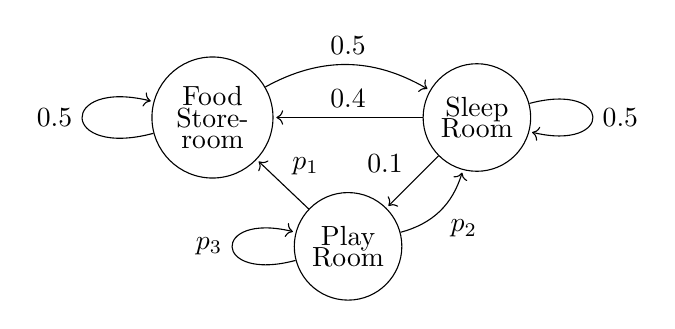
\begin{tikzpicture}[shorten >=1pt,node distance=0.5cm]
                \node[state, draw=none] (hidden) {};
                \node[state, left=of hidden, align=center] (fs) {Food \\[-1ex] Store-\\[-1ex]room};
                \node[state, right=of hidden, align=center] (sr) {Sleep \\[-1ex] Room};
                \node[state, below=of hidden, align=center] (pr) {Play \\[-1ex] Room};
                \draw[every loop]
                    (fs) edge[loop left] node{0.5} (fs)
                    (sr) edge[loop right] node{0.5} (sr)
                    (pr) edge[loop left] node{$p_3$} (pr)
                    (fs) edge[bend left, auto=left] node{0.5} (sr)
                    (sr) edge[auto=right] node{0.4} (fs)
                    (pr) edge[auto=right]  node{$p_1$}(fs)
                    (sr) edge[auto=right] node{0.1} (pr)
                    (pr) edge[auto=right, bend right] node{$p_2$} (sr);
            \end{tikzpicture}
        \end{center}
        (a) Let the number of furballs in each room (Food Storeroom, Sleep Room, and Play Room) at time $n$ be $x_f[n]$, $x_s[n]$, and $x_p[n]$, respectively. We would like to find the \textbf{transition matrix} $A$ such that 
        \begin{align*}
            \begin{bmatrix}
                x_f[n + 1] \\
                x_s[n + 1] \\
                x_p[n + 1]
            \end{bmatrix} = A
            \begin{bmatrix}
                x_f[n] \\
                x_s[n] \\
                x_p[n]
            \end{bmatrix}
        \end{align*}
        Write $A$ using the numbers and variables in the diagram.
    }
\end{frame}

\begin{frame}{Page Rank [Solution]}
    \color{blue}{
        The \textbf{transition matrix} is
        \begin{align*}
            A = \begin{bmatrix}
                0.5 & 0.4 & p_1 \\
                0.5 & 0.5 & p_2 \\
                0 & 0.1 & p_3
            \end{bmatrix}
        \end{align*}
        Remember that the element at row $i$, column $j$ represents the number of furballs going from room $j$ to room $i$.
    }
\end{frame}

\begin{frame}{Page Rank}
    (b) We know that \textit{no furballs enter or leave} the configuration of tunnels shown above and that during the time you're observing the behavior, \textit{no furballs die or are born}. What \textbf{constraint} does this place on the values of $p_1, p_2, p_3$? Write your answer in \textit{equation form}.
\end{frame}

\begin{frame}{Page Rank [Solution]}
    (b) We know that \textit{no furballs enter or leave} the configuration of tunnels shown above and that during the time you're observing the behavior, \textit{no furballs die or are born}. What \textbf{constraint} does this place on the values of $p_1, p_2, p_3$? Write your answer in \textit{equation form}.\\[2ex]
    \color{blue}{
        No furballs enter or leave the system, so the \textbf{sum of each column must be 1}. So,
        \begin{align*}
            p_1 + p_2 + p_3 = 1
        \end{align*}
    }
\end{frame}

\begin{frame}{Page Rank}
    (c) Suppose we let $\vec{p} = \begin{bmatrix}
        p_1 \\ p_2 \\ p_3
    \end{bmatrix}$ and $\vec{x}[n] = \begin{bmatrix}
        x_f[n] \\ x_s[n] \\ x_p[n]
    \end{bmatrix}$, and that we are sure that $x_p[n]$ is nonzero. \\[2ex]
    Express $\vec{p}$ as a function of the numbers in the diagram. $\vec{x}[n]$, and $\vec{x}[n + 1]$. (\textit{Hint: what is the relationship between $\vec{x}[n + 1]$ and $\vec{x}[n]$?})
\end{frame}

\begin{frame}{Page Rank [Solution]}
    (c) Suppose we let $\vec{p} = \begin{bmatrix}
        p_1 \\ p_2 \\ p_3
    \end{bmatrix}$ and $\vec{x}[n] = \begin{bmatrix}
        x_f[n] \\ x_s[n] \\ x_p[n]
    \end{bmatrix}$, and that we are sure that $x_p[n]$ is nonzero. \\[2ex]
    Express $\vec{p}$ as a function of the numbers in the diagram. $\vec{x}[n]$, and $\vec{x}[n + 1]$. (\textit{Hint: what is the relationship between $\vec{x}[n + 1]$ and $\vec{x}[n]$?})

    \color{blue}{
        \begin{align*}
            \vec{p} = \frac{1}{x_p[n]} \Bigg(\vec{x}[n + 1] - x_f[n]
            \begin{bmatrix}
                0.5 \\ 0.5 \\ 0
            \end{bmatrix} - x_s[n]
            \begin{bmatrix}
                0.4 \\ 0.5 \\ 0.1
            \end{bmatrix}\Bigg)
        \end{align*}
    }
\end{frame}

\begin{frame}{Steady State}
    (a) Consider a 2x2 matrix $A$, where max(eigenvalues($A$)) $>$ 1. Is it possible for the system defined by $x(t + 1) = Ax(t)$ to be \textbf{stable} (i.e. non-exploding) for some initial $x$?
\end{frame}

\begin{frame}{Steady State [Solution]}
    (a) Consider a 2x2 matrix $A$, where max(eigenvalues($A$)) $>$ 1. Is it possible for the system defined by $x(t + 1) = Ax(t)$ to be \textbf{stable} (i.e. non-exploding) for some initial $x$? \\[2ex]

    \color{blue}{
        Yes, but only as long as there is \textbf{another eigenvalue such that abs(eigenvalue) $\leq$ 1}  and only for an \textbf{appropriate initial state $x_0$}
    }
\end{frame}

\begin{frame}{Steady State}
    (b) Given a \textbf{conservative} state transition matrix $A$, is it possible for $A$ to have \textbf{multiple eigenvectors} corresponding to the eigenvalue 1? \textit{What does it say about the system?}
\end{frame}

\begin{frame}{Steady State [Solution]}
    (b) Given a \textbf{conservative} state transition matrix $A$, is it possible for $A$ to have \textbf{multiple eigenvectors} corresponding to the eigenvalue 1? \textit{What does it say about the system?} \\[2ex]
    \color{blue}{
        Yes. There is a set of \textbf{linearly independent steady-state}s, and \textit{any linear combination of those states is stable}.
    }
\end{frame}


% out of scope
% \section{Diagonalization}

\begin{frame}{Diagonalization}
	    \begin{itemize}
	        \item The idea is that we want to change into a basis in which the system $A\vec{x} = \vec{y}$ is represented by a diagonal matrix. So how do we find such basis?
	        
	        \item Remember that for all eigenvalue-eigenvector pairs we have: $A\vec{v} = \lambda\vec{v}$
	        
	        \item Let’s use our eigenvectors as our basis. Doing so we obtain:
	        
	        $$\vec{x} = V\tilde{\vec{x}}, \vec{y} = V\tilde{\vec{y}}, \text{and} \Lambda\tilde{\vec{x}} = \tilde{\vec{y}}$$
	        
	        Where the upper-case lambda represents the diagonal matrix with eigenvalues on the diagonals.
	        
	        \item Transforming back to the standard basis, we get:
            
            $$A = V\Lambda{V^{-1}}$$
	    \end{itemize}
	\end{frame}
	
	\begin{frame}{Diagonalization Cont.}
	    \begin{itemize}
	        \item Let’s analyze this a bit further, why is it important to be able to do this?
            
            \item We see that diagonalizing the matrix makes the system much easier to solve, why? 
            
            \item Also, we see that there is a “home state” for every system of linearly independent equations, i.e. the space in which the system’s components are uncoupled.
	    \end{itemize}
	\end{frame}
	


\end{document}
